\documentclass[../main/main.tex]{subfiles}

% \toggletrue{student}
% \HideSolutionstrue

\raggedbottom

\makeatletter
\renewcommand{\@chapapp}{M\'ecanique quantique -- chapitre}
\makeatother

\begin{document}
\setcounter{chapter}{0}
\chapter{Introduction \`a la m\'ecanique quantique}
\label{ch:mecaq}

\section{Un peu d'histoire}
\label{sec:mqhistoire}
Dans notre vie quotidienne, nous interagissons avec des systèmes à une échelle
macroscopique, qu'on modélise assez correctement en physique par un assemblage
de systèmes à l'échelle mésoscopique. L'idée de trouver une brique élémentaire à
ce qui compose notre monde, qui nous donnerait des clés pour le comprendre en le
prédire en totalité, est naturellement une idée ancienne. Le concept premier
d'«~atome~», du grec \textit{atomos}, «~insécable~», pensé par Démocrite et
Épicure, traduisait cette brique fondamentale hypothétique. Cependant, l'accès
expérimental à cette potentielle réalité physique est resté difficile pendant
de nombreux siècles.
% TODO: Citation on connaîtrait tout le monde avec les CI~: Laplace.
\bigbreak
En attendant, la majeure partie du monde physico-chimique tel qu'on le concevait
a été étudié et décrit~: la mécanique des solides et la mécanique des fluides,
la thermodynamique et la thermochimie, les ondes sonores et l'optique
géométrique… mais les questions sur la nature profonde de certains phénomènes
restent ouvertes, et de vifs débats enflamment les plus grands esprits.
\bigbreak
Au début du \textsc{xx}\ieme\ siècle, la lumière échappe à cette compréhension
profonde. Les outils existant sont ceux de la mécanique de \textsc{Newton} (fin
du \textsc{XVII}\ieme\ siècle) et l'électromagnétisme de \textsc{Maxwell}
(milieu et fin du \textsc{XIX}\ieme\ siècle)~: c'est la physique
\textbf{classique}, description du monde alors très robuste et complètement
déterministe, donnant une raison infiniment claire à toute observation du monde
réel. Cependant, quelques expériences les mettent en défaut~:
\begin{itemize}[label=$\diamond$, leftmargin=10pt]
	\litem{L'effet photoélectrique}~: exposer une plaque métallique exposée à de
	la lumière permet d'en arracher des électrons. Cependant, et ce peu importe
	l'intensité du faisceau, aucun électron n'est arraché si la lumière en
	question est au-dessus d'une certaine longueur d'onde (couleur)~: l'éjection
	n'apparaît qu'en-dessous d'une longueur d'onde seuil $\lambda_0$, ce que la
	physique classique n'explique alors pas encore.
	\begin{figure}[h!]
		\centering
		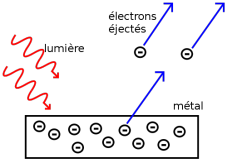
\includegraphics[scale=1]{photelec}
		\caption{Éjection des électrons d'un métal sous l'effet d'un faisceau
			lumineux.}
		\label{fig:photelec}
	\end{figure}
	\litem{Raies atomiques}~: en excitant un gaz d'un élément unique (comme
	l'hydrogène ou le néon) avec une tension électrique, le milieu dégage de la
	lumière. En la décomposant par un prisme, on obtient alors des raies très
	définies, à l'opposé des spectres continus qu'on observe généralement comme
	celui du soleil par exemple. Cette précision de longueur d'onde émise échappe
	à la physique classique.
	\begin{figure}[h!]
		\centering
		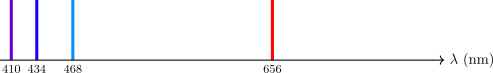
\includegraphics[scale=1]{raiesH-white}
		\caption{Spectre \textit{discret} des raies de l'hydrogène.}
		\label{fig:raiesH}
	\end{figure}
\end{itemize}
La résolution de ces incompréhensions va mener à la naissance de la mécanique
\textbf{quantique}, issu du latin \textit{quanta}, qui permet une
description des phénomènes physiques non pas comme un ensemble de phénomènes
continus, mais comme un ensemble de phénomènes \textbf{quantifiés}, notamment
\textit{via} des états d'énergie discrets et définis. Par exemple, c'est comme
si on pouvait aller à 50 \textbf{ou} \SI{70}{km.h^{-1}} en voiture, mais pas à
une valeur intermédiaire.
\bigbreak
Cette nouvelle approche du monde va bouleverser la façon de comprendre certains
phénomènes, et est à l'origine d'innombrables applications~: le laser, l'énergie
nucléaire, l'IRM, les semi-conducteurs et donc de toute l'électronique, mais
aussi toute la matière plus généralement et donc les interactions chimiques.

\section{Comportements ondulatoires}
\label{sec:mqonde}
\subsection{Diffraction}
\label{ssec:ondediff}
Une goutte d'eau seule ne fait pas une marrée~: c'est la collection d'objets
tangibles qui se meuvent de manière cohérente qui créé les vagues. On étudie
alors la vague comme un ensemble mais dont on comprend l'origine individuelle.
Une onde présente des propriétés particulières, dont une dont on a déjà parlé au
début de l'année~: la \textbf{diffraction}.
\begin{tdefi}{Définition~: diffraction}
	Lorsqu'une onde progressive rencontre un obstacle donc les dimensions sont de
	l'ordre de la longueur d'onde, la partie de l'onde qui la passe subit un
	\textbf{étalement circulaire}, qu'on appelle \textbf{diffraction}.
\end{tdefi}

\noindent
\begin{minipage}[t]{.5\linewidth}
	Une onde plane de longueur d'onde $\lambda$ arrivant sur une fente de taille
	$a \lesssim \lambda$ est diffractée \textit{majoritairement} dans un cône, de
	demi-angle d'ouverture
	\[
		\boxed{\sin{\theta} = \frac{\lambda}{a}}
	\]
	soit, pour des petits angles \textbf{en radians},
	\[
		\boxed{\tt \underset{\tt \ll 1}{\sim} \frac{\lambda}{a}}
	\]
\end{minipage}
\hfill
\begin{minipage}[t]{.45\linewidth}
	~
	\vspace*{-10pt}
	\begin{center}
		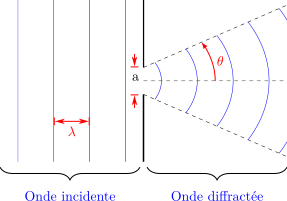
\includegraphics[width=.7\linewidth]{diff1d}
		\captionof{figure}{Diffraction par une fente. Les traits bleus représentent
			les maxima de l'onde.}
		\label{fig:diff1d}
	\end{center}
\end{minipage}

Ce comportement décrit très bien les ondes de matière comme les ondes sonores ou
les vagues arrivant dans un port, mais correspond également à ce que subit la
lumière en passant dans une fente~:
\begin{figure}[h]
	\centering
	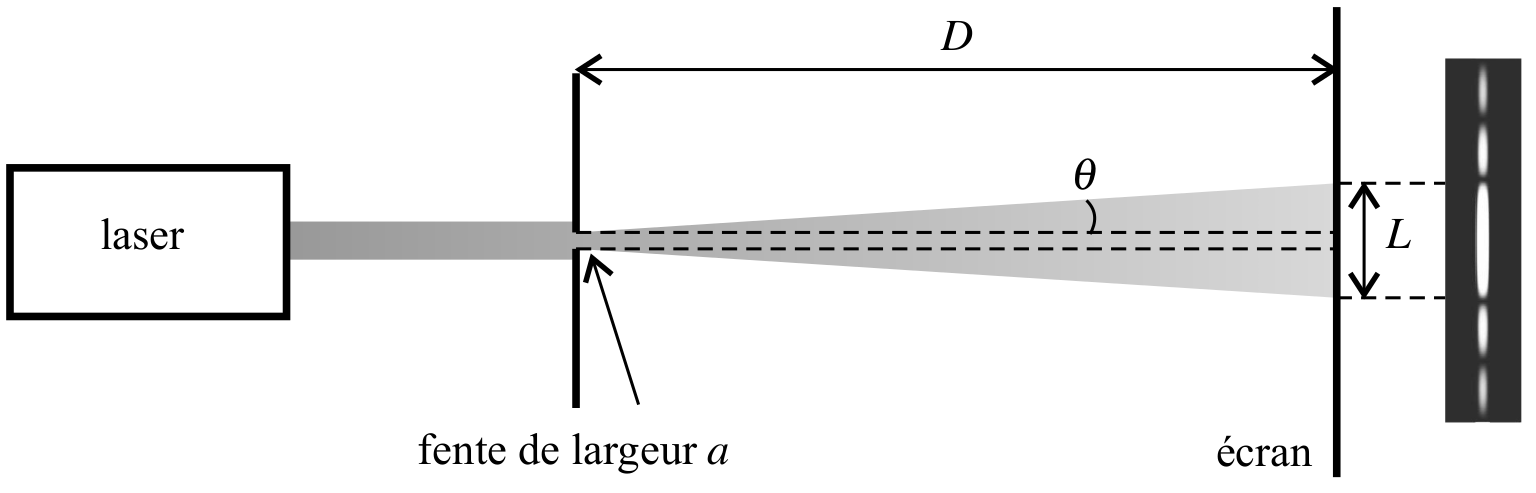
\includegraphics[width=.8\linewidth]{ch1_fig5}
	\caption{Diffraction d'un faisceau laser par une fente fine.}
	\label{fig:diff_las}
\end{figure}

\begin{rexem}{Application}
	Avec un laser de longueur d'onde $\lambda = \SI{630}{nm}$ et une fente de
	largeur $a = \SI{0.1}{mm}$, on observe sur l'écran placé à $D = \SI{5.0}{m}$
	une suite de taches de diffraction dont la plus large (au centre) est de
	largeur $L$. Calculer cette largeur.
	\tcblower
	On a $\sin{\theta} = \frac{\lambda}{a}$. Or, dans le triangle rectangle formé
	par le demi-cône entre la fente et l'écran, on a $\sin{\theta} =
		\frac{L/2}{D}$~; ainsi
	\begin{gather*}
		\frac{L}{2D} = \frac{\lambda}{a} \Lra \boxed{L = 2D \frac{\lambda}{a}}
		\\
		A.N.~: \ul{L = \SI{6.3}{cm}}
		\qav
		\begin{array}{ll}
			D       & = \SI{5.0}{m}
			\\
			\lambda & = \SI{630e-9}{m}
			\\
			a       & = \SI{0.1e-3}{m}
		\end{array}
	\end{gather*}
\end{rexem}

\subsection{Interférences}
\label{ssec:ondeint}
Une autre particularité des ondes est le phénomènes d'interférences~:
\begin{tdefi}{Définition~: interférence}
	Deux ondes de même nature se rencontrant en un point $\Mr$ se superposent en
	\textbf{sommant leurs signaux}.
\end{tdefi}
Nous avons également décrit ce phénomène plus tôt dans l'année, par l'expérience
des \textbf{fentes d'\textsc{Young}}.
\bigbreak
\noindent
\begin{minipage}{0.45\linewidth}
	La zone de l'espace où les faisceaux se superposent est appelé \textbf{champ
		d'interférences}. Sur un écran, on observe alors la figure ci-contre, avec
	des variations d'intensité lumineuse~:
	\begin{itemize}
		\item au milieu des zones claires (\textbf{maximum} local d'intensité)
		      on a des \textbf{interférences constructives}~;
		\item au milieu des zones sombres (\textbf{minimum} local d'intensité)
		      on a des \textbf{interférences destructives}.
	\end{itemize}
\end{minipage}
\hfill
\begin{minipage}{0.50\linewidth}
	\begin{center}
		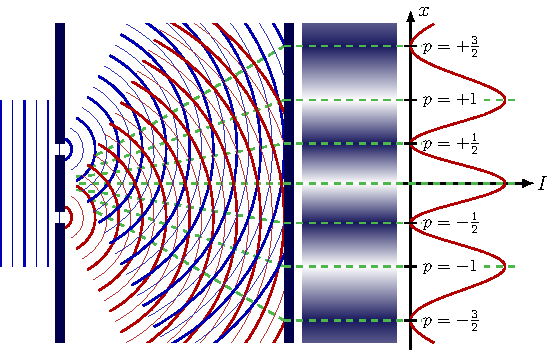
\includegraphics[width=\linewidth]{young_result}
	\end{center}
\end{minipage}

\begin{tror}{Conclusion, hand}
	Ainsi, il est clair que la lumière a un comportement ondulatoire. On peut donc
	songer que ce comportement est issu d'une collection d'objets individuels qui
	la composerait, des «~corpuscules~» de lumière~: les photons.
\end{tror}

\section{Dualité onde-corpuscule}
\label{sec:dualondcorp}

\subsection{Définitions}
\label{ssec:docdef}
\noindent
\begin{minipage}[t]{.45\linewidth}
	En physique classique (au \textsc{XIX}\ieme), le mouvmeent d'un…
	\begin{itemize}
		\item Un \textbf{corpuscule} est localisé
		\item Une \textbf{onde} n'est pas
	\end{itemize}

\end{minipage}
\hfill


\subsection{Nature corpusculaire de la lumière}
\label{ssec:lumcorp}
SCWHEITZER
\subsubsection{Photons}
\label{sssec:photons}
\subsubsection{Transitions atomiques}
\label{sssec:transatom}

\subsection{La matière~: onde et corpuscule.}
\label{ssec:matonde}

VIDEO Tout est quantique
\subsubsection{Rappels de mécanique classique}
\label{sssec:rapmeca}
OLIVIER

\subsubsection{Longueur d'onde de \textsc{de Broglie}}
\label{sssec:lgdb}
SCWHEITZER

\section{Formalisme quantique}
\label{sec:formQ}
SCWHEITZER, 1 et 2

\section{Relations d'incertitude d'\textsc{Heisenberg}}
\label{sec:heis}
OLIVIER

\section{Modèle semi-classique \textsc{Bohr}}
\label{sec:bohr}
SCWHEITZER

\end{document}
